% arara: xelatex
% arara: xelatex
% arara: xelatex


% options:
% thesis=B bachelor's thesis
% thesis=M master's thesis
% czech thesis in Czech language
% english thesis in English language
% hidelinks remove colour boxes around hyperlinks

\documentclass[thesis=B,english]{FITthesis}[2012/10/20]
\usepackage{threeparttable}

% \usepackage[utf8]{inputenc} % LaTeX source encoded as UTF-8
% \usepackage[latin2]{inputenc} % LaTeX source encoded as ISO-8859-2
% \usepackage[cp1250]{inputenc} % LaTeX source encoded as Windows-1250

\usepackage{graphicx} %graphics files inclusion
% \usepackage{subfig} %subfigures
% \usepackage{amsmath} %advanced maths
% \usepackage{amssymb} %additional math symbols
\usepackage[table,xcdraw]{xcolor}
\usepackage{dirtree} %directory tree visualisation
\usepackage{caption}
\usepackage{float}

% % list of acronyms
% \usepackage[acronym,nonumberlist,toc,numberedsection=autolabel]{glossaries}
% \iflanguage{czech}{\renewcommand*{\acronymname}{Seznam pou{\v z}it{\' y}ch zkratek}}{}
% \makeglossaries

% % % % % % % % % % % % % % % % % % % % % % % % % % % % % % 
% EDIT THIS
% % % % % % % % % % % % % % % % % % % % % % % % % % % % % % 

\department{Course: BI-SEP - World Economy and Business - B182}
\title{The connection between the number of teachers in elementary and secondary schools and the violent crimes rate in the USA.}
\authorGN{Roman} %author's given name/names
\authorFN{Levinzon} %author's surname
\author{Roman Levinzon} %author's name without academic degrees
\authorWithDegrees{Roman Levinzon} %author's name with academic degrees
\supervisor{PhDr. Ing. Tom{\' a}{\v s} Evan, Ph.D.}
\abstractEN{This working paper explores the connection between the number of teachers in elementary and secondary schools and the violent crimes rate on the example of the United States of America from 1997 to 2016. The hypothesis presented in this working paper suggests that there is a strong connection between these two values. The primary goal of this working paper is to analyze this connection and, using statistics data obtained from the official sources, to either prove the hypothesis or falsify it.

Through a regression analysis data from rom the U.S Department of Education and U.S Criminal Justice Information is examined to either accept the hypothesis or reject it.

The results of the analysis suggest there is a strong negative correlation between the number of teachers in elementary and secondary schools and the violent crime rate.}


\keywordsEN{USA, Violent crime rate, teachers, students, schools}


\let\cleardoublepage\clearpage

\begin{document}

% \newacronym{CVUT}{{\v C}VUT}{{\v C}esk{\' e} vysok{\' e} u{\v c}en{\' i} technick{\' e} v Praze}
% \newacronym{FIT}{FIT}{Fakulta informa{\v c}n{\' i}ch technologi{\' i}}

\setsecnumdepth{part}
\chapter{Introduction}
Human beings, among anything else, are violent creatures. We have been proving this to ourselves for centuries throughout human history. But there still something that distinguishes us from the animals, for whom the rule kill or be killed applies all the time, something that makes us humane. Since we are born, we always have someone by our side, someone who shows us the way the world works, teaches us how to make better decisions and solve problems along the way. We are constantly reminded that we are not alone in this world and the choices we make have consequences. Parents and teachers, among anyone else, are in the frontlines to guide us, especially in the young age. And one of the most significant part of this journey are elementary and secondary schools.

Education received in elementary and secondary schools, is more than solving basic math equations. Slowly but thoroughly, it teaches young kids how the modern world works, how it worked it before.  It helps them to socialize, to learn how to collaborate, teaches about the rights and wrongs. Considering the time a young student spends in there, this school becomes almost like a second family. 

Although, not every child is that lucky. There is always some number of children that do not have the privilege of attending these places, likely because some school could be private, meaning the education there is paid, or public with limited capacity.  It is even more common to see overcrowded classrooms with more than 30 children, as there are not enough teachers available.What happens then? The fact that the teacher got a huge number of students attending means he got much less chance to connect with them all, hence student pays less attention and loses interest in the topic. This then can result in a situation where the student would rather do something else instead of attending school, which often can lead towards a dark path.

This brings us to a primary hypothesis of this paper: I suggest that increasing the number of teachers in elementary and secondary would  decrease the violent crime rate.

\section{Goal}
The goal of this paper is to examine the relation between the independent variable
Number of teachers in schools  and the dependent variable violent crime rate in the USA from 1997 to
2016 and furthermore trying to prove the Hypothesis that these to values are negativelty related (i.e. increased value of independent variable will decrease the value of dependent variable). To achieve this, the data from the
U.S Department of Education \cite{tableteacher} and U.S Criminal Justice Information \cite{tablecrime} will be analyzed through the means of linear regression and prior research on this matter will be taken into consideration. The time frame observed is set from 1996 to 2016, because of the violent crime rate data availability. The United State of America was chosen as the country to be observed, because of how education system in there strongly affects the crime activity and how it is often very connected to each other.  

\section{Hypothesis Establishment}
It is important to establish all the variables that will be analyzed and verification criterias upon which the hypothesis will be tested.
\subsection{Hypothesis}
An increased number of teachers in secondary and elementary schools will result in lower violent crimes rate.

$H_0$ - There is no correlation between the number of teachers and the violent crimes rate.

$H_1$ - There is a correlation between the number of teachers and the violent crimes rate.

\subsection{Verification Criteria}
$R^2 > 0.75$ and Correlation  $< -0,75$

\noindent $p$ - value is less than $0,05$ (Confidence interval of 95\%).

 
\textbf{Independent Variable:} The number of teachers in elementary and secondary schools

\textbf{Dependent Variable:} The violent crimes rate

\setsecnumdepth{all}
\chapter{Theoretical part}

This chapter serves as a theoretical background for the problem in question. It explores the role of education, how it affects the children's future and explores its possible connection to a criminal activities preparing the roots for the hypothesis proof.

\section{The Role of Education}
One of the most influent English philosophers, John Lock, one called a mind of the child a "white paper" and that all of our knowledge believes and ideas are derived from the experience \cite{lockey2}. Children mind is considered one the easiest to influent and impact; that is why it is crucial how the child is educated. Nowadays it is the elementary school and secondary schools are playing a big role in overall education.


Elementary school forms the foundation of what we are. Here we gain a basic understanding of how to gain knowledge. It offers a stable group of individuals for children to interact with, so the child can learn about how to make personal decisions, find his place in the society and set personal goals along the way. And usually, the skills and the attitude we obtain in this period serves as the foundation for future successes \cite{education}. On top of it all, of course, are teachers and parents. Let's explore the teacher's role to support our theory.

\section{Teacher And The Students}

Judging by the amount the child is spending in the school, the teacher has an immense impact on his students.  John Lock even compares the tutor to a second father figure, arguing that is the second person that child should spend most his/her time with, right after the parents \cite{locke2013some}. And being the teacher is more than a job -- it is a calling. Being a teacher requires you not only being able to teach the subject in question but also to be able to develop an interest in the topic, guide your pupils and be able to help in time of need.  Greek philosopher Plutarch once said that student's mind not the vessel that needs to be filled, but rather a torch that must be ignited. And only the person that is ignited as well can do it \cite{pluto}. So the good teacher not only leads to more educated youth but also adds to the school culture overall.

And, as mentioned before, the knowledge itself is not the only thing that is school and teacher provides. It is also a place where student makes new friends and starts to act as part of the society. Being the teacher, gives you an ability  to prevent people from making mistakes and to encourage them to become productive members of society.


\section{Education and Crime Activity}
What is the origin of criminal activity? According to the working paper of Erling Eide, Paul Rubin, and  Joanna Shepherd, well-to-do people are less likely to commit a crime.  In their work, they discuss two main factors that are most likely to be the root of the problem: Income inequality and unemployment \cite{crimeeco}.

Both of these factors, while they can be caused by a vast amount of different other issues, there are a lot of researches that easily connect these two factors with education. For example, Jacob Mincer in his work "Education And Employment" \cite{employment} explores this connection and determines that this connection appears to be straightforward and negative. He is arguing that not only that the education provides the benefit of the stability, but the educated people, in general, tend to invest more time in training and professional growth, which lead to shorter off-the-job search periods.

Another issue, that is very common in the USA and can lead towards a criminal activity is bullying, and it got even more attention during past fifteen years. Study of 2007 by Andre Sourander and his team \cite{bulying}, indicates that both bullies and the ones being bullied are then more likely to commit a crime. The results showed that 9\% of the bullying victims and 15.9\% of the bullies committed more than 2 crimes at ages 16 to 20 years, as opposed to children that were not bullied so much: 6.8\%.



\section{Number of Teachers}
We have established to main problems that connects education ad criminal activity: unemployment and income inequality and bullying. How the teachers number can affect it?

\subsection{Education Inefficiency}
Both unemployment and income inequality can be caused by eduction inefficiency. When education is inefficient and how it can be improved?


Sometimes there are just no enough teachers. This could either lead to an oversized classrooms or for one teacher to work twice as hard. In both cases it makes it hard for the teacher to pay enough attention to all his students, some of which may be problematic. On the other hand, in oversized classrooms in particular, a student  looses an already small amount of attention ever more quickly.  That is the exact problem that John Lock describes in his other work \cite{locke2013some}. He says how crucial it is  to have a students attention and that schools, in general, do not achieve this goal due to the amount pupils attending \cite{locke2013some}.

 The most popular point of view on this topic is that smaller classroom size gives more time for a teacher to address the issues of individual students. And some studies support this statement.  Soo Shin and Jae Young Chung in their study \cite{classsize} tried to analyze how the number of students in class affects their academic performance -- Class Size Reduction (CSR) -- which is usually done by increasing the number of teachers.
 
 Though they stated that there are a lot of different factors that affect students' success (like school culture or teacher's skill level), overall, the student achievement of the small classes turned out to be better than that of students in large classes by 0.20 standard deviations. What is even more critical for our research is that the CRS approach is the most effective in the early stage of studentship -- elementary school especially. 
 
 \subsection{Bullying prevention is the Crime Prevention}
 
 
It is the teachers' responsibility to act as a role model and serve as an example for their students. And, when it comes to bullying teacher must at all costs try to prevent such behavior, because, as we established, it can result in something much worse than just bullying.  An increased amount of teachers might help this situation as well, as it will be easier for the teachers to be aware of their students' mindset and conflicts.

 

 
\section{Chapter Summary}

So long we have been discussing the overall impact of the education system on a human being, especially in the young age. We have established, that the teacher figure plays one of the important roles in the education process, and that the increased number of teachers might have a positive impact on students future.

 Some of researches and studies can actually support our hypothesis but in order to actually accept or reject our hypothesis the practical part must be completed first.
\floatstyle{plaintop}
\restylefloat{table}
\chapter{Practical Part}
This chapter will further analyze the problem in question and try to prove the hypothesis  using the means of linear regression based on the data sample.

\section{Proving The Hypothesis}
Table \ref{tab:teacher} shows data for our Independent variable (i.e the number of teachers in secondary and elementary schools) and Table \ref{tab:violence} contains a data for our Dependent variable(i.e violent crime rate). Both data samples are from the same time period: 1997-2016. Based on these tables, Figure 2.1 demonstrates the regression analysis of our two variables showing the relation between them. 

 The correlation between the two variables is $-0.952736534$. As a correlation of -1 means there is
perfect negative correlation between two variables, we can deduce that with a correlation of
$-0.952736534$ these two variables show a significant negative correlation. The value of $R^2$ being
0.9077  suggest further evidence for the strong correlation between the number of teachers and the violent crime rate. The $p$ - value of 9,41113035408523E-11 suggests that these results are rather
significant and are quite strong within the proposed confidence interval of 95\%. 

Based on these
results we can reject $H_0$-hypothesis and accept $H_1$-hypothesis.

\newpage
\begin{table}[H]
\def\arraystretch{1.7}%  1 is the default, change whatever you need
\captionsetup{justification=centering}
\begin{tabular}{|c|c|}
\hline
\textbf{Year} & \textbf{Number Of Teachers in Secondary and Elementary Schools} \\ \hline
1997          & 3138                                                            \\ \hline
1998          & 3230                                                            \\ \hline
1999          & 3319                                                            \\ \hline
2000          & 3366                                                            \\ \hline
2001          & 3440                                                            \\ \hline
2002          & 3476                                                            \\ \hline
2003          & 3490                                                            \\ \hline
2004          & 3538                                                            \\ \hline
2005          & 3593                                                            \\ \hline
2006          & 3622                                                            \\ \hline
2007          & 3634                                                            \\ \hline
2008          & 3689                                                            \\ \hline
2009          & 3705                                                            \\ \hline
2010          & 3725                                                            \\ \hline
2011          & 3763                                                            \\ \hline
2012          & 3812                                                            \\ \hline
2013          & 3867                                                            \\ \hline
2014          & 3933                                                            \\ \hline
2015          & 4001                                                            \\ \hline
2016          & 4069                                                            \\ \hline
\end{tabular}
\caption{Number of Teacher in Elementary and Secondary Schools from 1997 to 2016 \cite{tableteacher}}
\label{tab:teacher}
\end{table}
\setsecnumdepth{part}


\begin{table}[H]
\centering
\def\arraystretch{1.7}%  1 is the default, change whatever you need
\captionsetup{justification=centering}
\begin{tabular}{|c|c|}
\hline
\textbf{Year} & \textbf{Violent Crime Rate per 100000 Inhabitants in USA} \\ \hline
1997          & 611                         \\ \hline
1998          & 567,6                       \\ \hline
1999          & 523                         \\ \hline
2000          & 506,5                       \\ \hline
2001          & 504,5                       \\ \hline
2002          & 494,4                       \\ \hline
2003          & 475,8                       \\ \hline
2004          & 463,2                       \\ \hline
2005          & 469                         \\ \hline
2006          & 479,3                       \\ \hline
2007          & 471,8                       \\ \hline
2008          & 458,6                       \\ \hline
2009          & 431,9                       \\ \hline
2010          & 404,5                       \\ \hline
2011          & 387,1                       \\ \hline
2012          & 387,8                       \\ \hline
2013          & 369,1                       \\ \hline
2014          & 361,6                       \\ \hline
2015          & 373,7                       \\ \hline
2016          & 386,3                       \\ \hline
\end{tabular}
\caption{Violent crimes rate in USA from year 1997 to 2016 \cite{tablecrime} }
\label{tab:violence}
\end{table}


\begin{figure}[H]
	\label{fig:graph}
	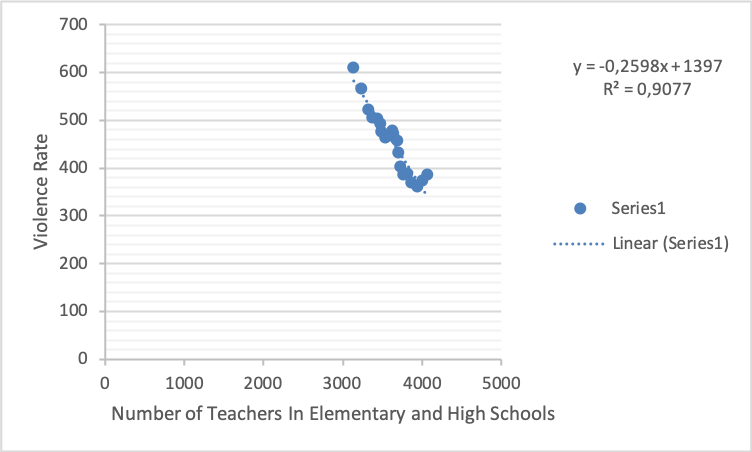
\includegraphics{graph}
	\caption{Regression Analysis: Number  of teachers and Violent Crime Rate}
\end{figure}


\noindent Slope = $-0.2598$ \newline \newline
Correlation = $-0,952736534$ \newline \newline
$R^2$ = 0.9077 \newline \newline
$F(Y) =-0.2598x - 1397$ \newline \newline
$p$ - value = $9,41113035408523E-11$


\chapter{Conclusion}

The practical part of this working paper shows the support for the thesis that our two variables (the number of teachers in secondary and elementary schools, and the violent crime rates) are related to each other, and one impacts the other. Furthermore, the relation between the two variables can be examined to be negatively correlated. The calculated correlation is  $-0,952736534$  and $R^2$ is  0.9077. The $p$ - value was found to be 9,41113035408523E-11, being well within the confidence interval, which leads
to the acceptance of the $H_1$ - hypothesis. 


These results lead to the conclusion that the number of teachers in elementary and secondary schools could be one of the critical factors that causing  may affect the violent crime rate in the USA. However, there is no doubt that there are other factors shout be taken into to be taken into account to create more accurate statement about this relationship. 

Future research could take these factors into account to make the statement more precise.



\bibliographystyle{iso690}
\bibliography{mybibliographyfile}

\setsecnumdepth{all}
\appendix

\chapter{Acronyms}
% \printglossaries
\begin{description}
	\item[GUI] Graphical user interface
	\item[XML] Extensible markup language
\end{description}


\chapter{Contents of enclosed CD}

%change appropriately

\begin{figure}
	\dirtree{%
		.1 readme.txt\DTcomment{the file with CD contents description}.
		.1 exe\DTcomment{the directory with executables}.
		.1 src\DTcomment{the directory of source codes}.
		.2 wbdcm\DTcomment{implementation sources}.
		.2 thesis\DTcomment{the directory of \LaTeX{} source codes of the thesis}.
		.1 text\DTcomment{the thesis text directory}.
		.2 thesis.pdf\DTcomment{the thesis text in PDF format}.
		.2 thesis.ps\DTcomment{the thesis text in PS format}.
	}
\end{figure}

\end{document}
